\documentclass[aspectratio=169,professionalfonts, 12pt, t]{beamer}
\usepackage{lmodern}

\newcommand{\presentationTitle}{Développement d'une approche de distribution des espaces d'états basé sur la théorie de jeux : \\Application au model checking distribué}
\newcommand{\shortTitle}{\textbf{Approche de distribution des espaces d'états basé sur la théorie de jeu}}
\newcommand{\presentationSubtitle}{Ein Template für die \LaTeX{}-Klasse \enquote{Beamer}}
\newcommand{\university}{Université Constantine 2}
\newcommand{\universityCourse}{IFA}
\newcommand{\universityDepartment}{Faculté des Nouvelles Technologies \\Département d’Informatique Fondamentale et\\ ses Applications}
\newcommand{\presentationKeywords}{\LaTeX, Beamer}
\newcommand{\presentationAuthor}{Karimou Seyni Ibrahim}
\newcommand{\presentationAuthorShort}{Karimou.S.I}
\newcommand{\presentationAuthorEmail}{ibrahim.karimouseyni@yahoo.com}
\newcommand{\presentationSubject}{Informatique}
\newcommand{\presentationLocation}{Leipzig}

\title[\shortTitle]{\presentationTitle{}}
\subtitle{\presentationSubtitle}
\author[\presentationAuthorShort]{\large \presentationAuthor}
 
\date{\today} 

%
% XeTeX specific
%
%\RequireXeTeX
 \usepackage{xltxtra}
%\usepackage{fontspec}
%\usepackage{xunicode}

% -----------------------------------
% font config
% -----------------------------------

%\setsansfont{Linux Biolinum}
%\setromanfont{Linux Libertine}
%\setmonofont[Scale=0.9]{Consolas}

% -----------------------------------
% math
% -----------------------------------
\usepackage{lmodern}

\usepackage[utf8]{inputenc} % this is needed for german umlauts
\usepackage[ngerman]{babel} % this is needed for german umlauts
\usepackage[T1]{fontenc}    % this is needed for correct output of umlauts in pdf

\usepackage{amsmath}
\usepackage{amsfonts}
\usepackage{amssymb}
\usepackage{amsthm}
\usepackage{mathrsfs}   % \mathscr
\usepackage{stmaryrd}   % \lightning

% -----------------------------------
% grammar and textstyle
% -----------------------------------

\usepackage{polyglossia}
\setdefaultlanguage{german}
\usepackage{csquotes}
% underlining
\usepackage{soul} % ulem redifines \emph, this sucks

% -----------------------------------
% colors
% -----------------------------------

\usepackage{xcolor}
\usepackage{colortbl}

% listing colors
% https://kuler.adobe.com/Color-palette-color-theme-4004722
\definecolor{keyword}{RGB}{239,33,74}
\definecolor{number}{RGB}{243,202,22}
\definecolor{comment}{RGB}{126,158,19}
\definecolor{string}{RGB}{6,129,128}
\usepackage{fontawesome}
 

\usepackage{tikz}
\usetikzlibrary{positioning, arrows}
\usepackage{animate}
\usepackage{graphicx}
% -----------------------------------
% links and references
% -----------------------------------

\usepackage{hyperref}
\hypersetup{
    colorlinks=false,
    % hide bookmarks
    pdfpagemode=UseNone,
    % meta
    pdfauthor={\presentationAuthor},
    pdftitle={\presentationTitle}
}
\usepackage[german]{cleveref}

% -----------------------------------
% bibliography and glossaries
% -----------------------------------

\usepackage[
    backend=biber,
    style=alphabetic-verb
    ]{biblatex}
\bibliography{presentation}

\usepackage{glossaries}
\input{glossary}
\makeglossaries

% -----------------------------------
% graphics
% -----------------------------------

\usepackage{graphicx}
\usepackage{tikz}
\usetikzlibrary{shapes.geometric, arrows, shadows, positioning}
\usepackage{adforn} % ornaments, used in titlepage
\usepackage{multicol}
% -----------------------------------
% beamer theme
% -----------------------------------

% you can't locate the theme in a subfolder without shooting yourself in the knee
\usetheme{alinz}

% -----------------------------------
% listings and pseudocode
% -----------------------------------

\Crefname{lstlisting}{Listing}{Listings}
\crefname{lstlisting}{listing}{listings}

\usepackage{listings}
\lstset{
    basicstyle=\footnotesize\ttfamily\color{lightdark},
    backgroundcolor=\color{blockbg},
    numbers=left,
    %numbersep=6pt,
    numberstyle=\scriptsize\color{granite},
    commentstyle=\sffamily\itshape\color{sea},
    keywordstyle=\bfseries\color{raspberry},
    stringstyle=\itshape\color{lake},
    showstringspaces=false,
    breaklines=true,
    breakatwhitespace=true,
    frame=lr,
    framerule=0pt,
    framesep=6pt,
    captionpos=b
}
% for pseudocode
\usepackage[slide,linesnumbered,algoruled]{algorithm2e}
\usepackage{pst-plot}
\usepackage{pst-solides3d}
\xdefinecolor{pgold}{rgb}{0.8,0.6,0.2}

\psset{viewpoint=50 20 10 rtp2xyz,Decran=50,linewidth=0.5\pslinewidth}
% These next six lines declare a new beamerboxes environment
%\setbeamercolor{uppercol}{ffg=blocktitlefg, bg=titlebg}
\setbeamercolor{lowercol}{fg=lightdark, bg=blockbg}
\newenvironment{colorblock}
{
	\begin{beamerboxesrounded}[lower=lowercol,shadow=true]}
	{\end{beamerboxesrounded}}

\usetikzlibrary{arrows,shapes}
\usepackage{verbatim}
% Define some styles for graphs
\tikzstyle{vertex}=[circle,fill=black!25,minimum size=20pt,inner sep=0pt]
\tikzstyle{selected vertex} = [vertex, fill=red!24]
\tikzstyle{blue vertex} = [vertex, fill=blue!24]
\tikzstyle{edge} = [draw,thick,-]
\tikzstyle{weight} = [font=\small]
\tikzstyle{selected edge} = [draw,line width=5pt,-,red!50]
\tikzstyle{ignored edge} = [draw,line width=5pt,-,black!20]


% http://tex.stackexchange.com/questions/99500/listings-code-style-for-html5-css-html-javascript
\lstdefinelanguage{JavaScript}{
    morekeywords={break, case, catch, continue, debugger, default, delete, do, else, false, finally, for, function, if, in, instanceof, new, null, return, switch, this, throw, true, try, typeof, var, void, while, with},
    morecomment=[s]{/*}{*/},
    morecomment=[l]//,
    morestring=[b]",
    morestring=[b]'
}

% http://tex.stackexchange.com/questions/99500/listings-code-style-for-html5-css-html-javascript
\lstdefinelanguage{HTML5}{
        language=html,
        sensitive=true,
        alsoletter={<>=-},
        otherkeywords={
        % HTML tags
        < </, >,
        </a, <a, </a>,
        </abbr, <abbr, </abbr>,
        </address, <address, </address>,
        </area, <area, </area>,
        </area, <area, </area>,
        </article, <article, </article>,
        </aside, <aside, </aside>,
        </audio, <audio, </audio>,
        </audio, <audio, </audio>,
        </b, <b, </b>,
        </base, <base, </base>,
        </bdi, <bdi, </bdi>,
        </bdo, <bdo, </bdo>,
        </blockquote, <blockquote, </blockquote>,
        </body, <body, </body>,
        </br, <br, </br>,
        </button, <button, </button>,
        </canvas, <canvas, </canvas>,
        </caption, <caption, </caption>,
        </cite, <cite, </cite>,
        </code, <code, </code>,
        </col, <col, </col>,
        </colgroup, <colgroup, </colgroup>,
        </data, <data, </data>,
        </datalist, <datalist, </datalist>,
        </dd, <dd, </dd>,
        </del, <del, </del>,
        </details, <details, </details>,
        </dfn, <dfn, </dfn>,
        </div, <div, </div>,
        </dl, <dl, </dl>,
        </dt, <dt, </dt>,
        </em, <em, </em>,
        </embed, <embed, </embed>,
        </fieldset, <fieldset, </fieldset>,
        </figcaption, <figcaption, </figcaption>,
        </figure, <figure, </figure>,
        </footer, <footer, </footer>,
        </form, <form, </form>,
        </h1, <h1, </h1>,
        </h2, <h2, </h2>,
        </h3, <h3, </h3>,
        </h4, <h4, </h4>,
        </h5, <h5, </h5>,
        </h6, <h6, </h6>,
        </head, <head, </head>,
        </header, <header, </header>,
        </hr, <hr, </hr>,
        </html, <html, </html>,
        </i, <i, </i>,
        </iframe, <iframe, </iframe>,
        </img, <img, </img>,
        </input, <input, </input>,
        </ins, <ins, </ins>,
        </kbd, <kbd, </kbd>,
        </keygen, <keygen, </keygen>,
        </label, <label, </label>,
        </legend, <legend, </legend>,
        </li, <li, </li>,
        </link, <link, </link>,
        </main, <main, </main>,
        </map, <map, </map>,
        </mark, <mark, </mark>,
        </math, <math, </math>,
        </menu, <menu, </menu>,
        </menuitem, <menuitem, </menuitem>,
        </meta, <meta, </meta>,
        </meter, <meter, </meter>,
        </nav, <nav, </nav>,
        </noscript, <noscript, </noscript>,
        </object, <object, </object>,
        </ol, <ol, </ol>,
        </optgroup, <optgroup, </optgroup>,
        </option, <option, </option>,
        </output, <output, </output>,
        </p, <p, </p>,
        </param, <param, </param>,
        </pre, <pre, </pre>,
        </progress, <progress, </progress>,
        </q, <q, </q>,
        </rp, <rp, </rp>,
        </rt, <rt, </rt>,
        </ruby, <ruby, </ruby>,
        </s, <s, </s>,
        </samp, <samp, </samp>,
        </script, <script, </script>,
        </section, <section, </section>,
        </select, <select, </select>,
        </small, <small, </small>,
        </source, <source, </source>,
        </span, <span, </span>,
        </strong, <strong, </strong>,
        </style, <style, </style>,
        </summary, <summary, </summary>,
        </sup, <sup, </sup>,
        </svg, <svg, </svg>,
        </table, <table, </table>,
        </tbody, <tbody, </tbody>,
        </td, <td, </td>,
        </template, <template, </template>,
        </textarea, <textarea, </textarea>,
        </tfoot, <tfoot, </tfoot>,
        </th, <th, </th>,
        </thead, <thead, </thead>,
        </time, <time, </time>,
        </title, <title, </title>,
        </tr, <tr, </tr>,
        </track, <track, </track>,
        </u, <u, </u>,
        </ul, <ul, </ul>,
        </var, <var, </var>,
        </video, <video, </video>,
        </wbr, <wbr, </wbr>,
        />, <!
        },
        ndkeywords={
        % General
        =,
        % HTML attributes
        accept=, accept-charset=, accesskey=, action=, align=, alt=, async=, autocomplete=, autofocus=, autoplay=, autosave=, bgcolor=, border=, buffered=, challenge=, charset=, checked=, cite=, class=, code=, codebase=, color=, cols=, colspan=, content=, contenteditable=, contextmenu=, controls=, coords=, data=, datetime=, default=, defer=, dir=, dirname=, disabled=, download=, draggable=, dropzone=, enctype=, for=, form=, formaction=, headers=, height=, hidden=, high=, href=, hreflang=, http-equiv=, icon=, id=, ismap=, itemprop=, keytype=, kind=, label=, lang=, language=, list=, loop=, low=, manifest=, max=, maxlength=, media=, method=, min=, multiple=, name=, novalidate=, open=, optimum=, pattern=, ping=, placeholder=, poster=, preload=, pubdate=, radiogroup=, readonly=, rel=, required=, reversed=, rows=, rowspan=, sandbox=, scope=, scoped=, seamless=, selected=, shape=, size=, sizes=, span=, spellcheck=, src=, srcdoc=, srclang=, start=, step=, style=, summary=, tabindex=, target=, title=, type=, usemap=, value=, width=, wrap=,
        % CSS properties
        accelerator:,azimuth:,background:,background-attachment:,
        background-color:,background-image:,background-position:,
        background-position-x:,background-position-y:,background-repeat:,
        behavior:,border:,border-bottom:,border-bottom-color:,
        border-bottom-style:,border-bottom-width:,border-collapse:,
        border-color:,border-left:,border-left-color:,border-left-style:,
        border-left-width:,border-right:,border-right-color:,
        border-right-style:,border-right-width:,border-spacing:,
        border-style:,border-top:,border-top-color:,border-top-style:,
        border-top-width:,border-width:,bottom:,caption-side:,clear:,
        clip:,color:,content:,counter-increment:,counter-reset:,cue:,
        cue-after:,cue-before:,cursor:,direction:,display:,elevation:,
        empty-cells:,filter:,float:,font:,font-family:,font-size:,
        font-size-adjust:,font-stretch:,font-style:,font-variant:,
        font-weight:,height:,ime-mode:,include-source:,
        layer-background-color:,layer-background-image:,layout-flow:,
        layout-grid:,layout-grid-char:,layout-grid-char-spacing:,
        layout-grid-line:,layout-grid-mode:,layout-grid-type:,left:,
        letter-spacing:,line-break:,line-height:,list-style:,
        list-style-image:,list-style-position:,list-style-type:,margin:,
        margin-bottom:,margin-left:,margin-right:,margin-top:,
        marker-offset:,marks:,max-height:,max-width:,min-height:,
        min-width:,transition-duration:,transition-property:,
        transition-timing-function:,transform:,
        -moz-transform:,-moz-binding:,-moz-border-radius:,
        -moz-border-radius-topleft:,-moz-border-radius-topright:,
        -moz-border-radius-bottomright:,-moz-border-radius-bottomleft:,
        -moz-border-top-colors:,-moz-border-right-colors:,
        -moz-border-bottom-colors:,-moz-border-left-colors:,-moz-opacity:,
        -moz-outline:,-moz-outline-color:,-moz-outline-style:,
        -moz-outline-width:,-moz-user-focus:,-moz-user-input:,
        -moz-user-modify:,-moz-user-select:,orphans:,outline:,
        outline-color:,outline-style:,outline-width:,overflow:,
        overflow-X:,overflow-Y:,padding:,padding-bottom:,padding-left:,
        padding-right:,padding-top:,page:,page-break-after:,
        page-break-before:,page-break-inside:,pause:,pause-after:,
        pause-before:,pitch:,pitch-range:,play-during:,position:,quotes:,
        -replace:,richness:,right:,ruby-align:,ruby-overhang:,
        ruby-position:,-set-link-source:,size:,speak:,speak-header:,
        speak-numeral:,speak-punctuation:,speech-rate:,stress:,
        scrollbar-arrow-color:,scrollbar-base-color:,
        scrollbar-dark-shadow-color:,scrollbar-face-color:,
        scrollbar-highlight-color:,scrollbar-shadow-color:,
        scrollbar-3d-light-color:,scrollbar-track-color:,table-layout:,
        text-align:,text-align-last:,text-decoration:,text-indent:,
        text-justify:,text-overflow:,text-shadow:,text-transform:,
        text-autospace:,text-kashida-space:,text-underline-position:,top:,
        unicode-bidi:,-use-link-source:,vertical-align:,visibility:,
        voice-family:,volume:,white-space:,widows:,width:,word-break:,
        word-spacing:,word-wrap:,writing-mode:,z-index:,zoom:
        },
        morecomment=[s]{<!--}{-->},
        tag=[s]
}


%\usepackage[utf8]{inputenc} % this is needed for german umlauts
%\usepackage[ngerman]{babel} % this is needed for german umlauts
%\usepackage[T1]{fontenc}    % this is needed for correct output of umlauts in pdf

\usepackage{verbatim}
\usepackage{tikz}
\usetikzlibrary{arrows,shapes}

% see http://deic.uab.es/~iblanes/beamer_gallery/index_by_theme.html
%\usetheme{Frankfurt}
\usetheme{alinz}
%\usepackage[frenchb]{babel}
%\usepackage[T1]{fontenc}
%\usepackage[utf8]{inputenc}

% \usetheme{default} -> A utiliser dans un premier temps
% \usetheme{Warsaw} -> A utiliser dans un second temps
% position the logo
 \jurya{Pr. Djamel Eddine SAIDOUNI}{Directeur de mémoire}{}
 \juryb{Dr. Bouneb Zine El Abidine}{Co-encadreur}{}


%\title[Faire une présentation en LaTeX avec Beamer]{\LARGE Développement d'une approche de distribution des espaces d'états basé sur la théorie de jeux : Application au model checking distribué}
%\author{Spader}
%\institute{www.siteduzero.com}
%\date{\today}
\begin{document}
	\begin{frame}[plain, t,noframenumbering]
	\titlepage
	\end{frame}
\begin{frame}[plain,noframenumbering]
\frametitle{SOMMAIRE}
\tableofcontents
\end{frame}

	\section{Introduction}

\subsection{Definition}
\begin{frame}{Définition}
    \begin{block}{formales System}
        Ein System welches Regeln enthält, mit deren Hilfe sich mathematische Aussagen beweisen lassen und mit denen aus bereits bewiesenen Aussagen neue Aussagen abgeleitet werden können.
    \end{block}
    \begin{block}{widerspruchsfrei}
        \begin{itemize}
            \item $A$ Aussage
            \item $T$ formales System
        \end{itemize}
        $$\neg\exists A: T\rightarrow{}A \wedge T\rightarrow{}\neg{}A $$
    \end{block}
\end{frame}
	\section{Solutions Proposées}
%les solutions proposées dans la literature sont faites en amont, nous pouvons clasifier ces solutions en 2 categories
\subsection{Première Catégorie}
\begin{frame}{title sub section}
\begin{wrapfigure}{r}{0.3\textwidth}
	\vspace{-35pt}
	\begin{center}
		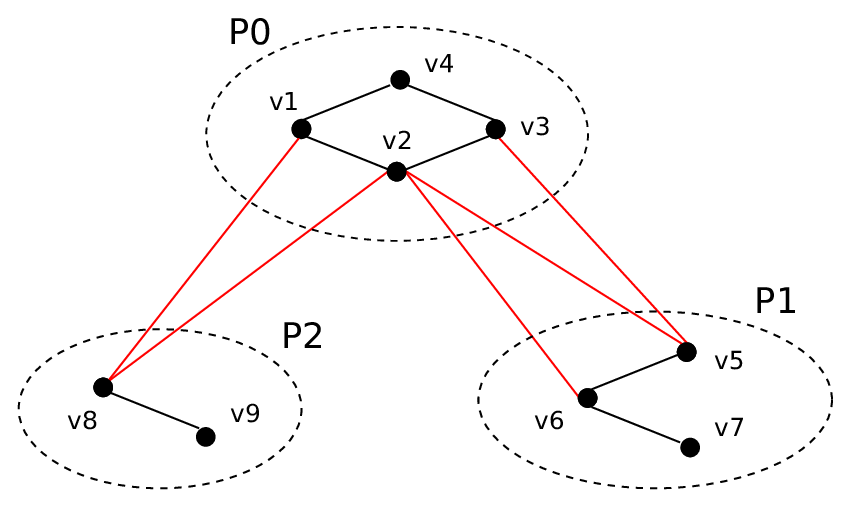
\includegraphics[width=0.2\textwidth]{resources/partitions}
	\end{center}
	\vspace{-35pt}
	\end{wrapfigure}
       Les approches de cette catégorie aboutissent à une meilleur équilibrage de charge entre les différentes machines.
		\begin{columns}
      		\begin{column}{0.3\textwidth}
      			\begin{figure}
      				\centering
      				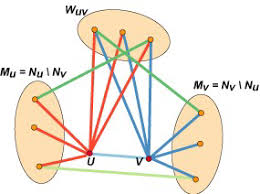
\includegraphics[width=\linewidth]{resources/transitions}
      			\end{figure}      			
      		\end{column}
      	
	      	\begin{column}{0.7\textwidth}
	      		\begin{block}{Problèmes}
	      			\begin{itemize}
	      				\item Distribution statique.% la distribution reste intacte tout au long du model cheking
	      				\item Nombre de Transitons externes minimum implique -t-il réduction du taux de communication?.% pourai entrainer un nombre elever de communications
	      				
	      				\item La puissance des machines non exploitée.% il peut y avoir des machines qui effetue peut de calcule alors que les autres un nombre elevé de calcul
	      				\item Temps de réponse déraisonnable.
	      			\end{itemize}
	      		\end{block}
	      	\end{column}
      	\end{columns}	    
\end{frame}

\subsection{Deuxième Catégorie}
\begin{frame}{title sub section}
\begin{wrapfigure}{r}{0.3\textwidth}
	\vspace{-20pt}
	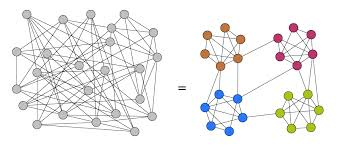
\includegraphics[width=0.3\textwidth]{resources/transition}
	\vspace{-20pt}
\end{wrapfigure}
La philosophie de cette catégorie vise à minimiser les transitions externes avec un bon équilibrage de charge entre les différentes machines.
 
		%\item Distribution statique.% la distribution reste intacte tout au long du model cheking
		\begin{columns}
			\begin{column}{0.3\textwidth}
				\centering
				\begin{figure}
					\begin{tikzpicture}		

						\node [inner sep=-10pt,visible on=<1-1>]{
							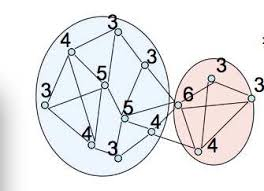
\includegraphics[height=1.2in,width=\columnwidth,trim={0 0 0 0},clip]{resources/bequilibre}
						};              
					
					\node [inner sep=-10pt,visible on=<2->]
					{
						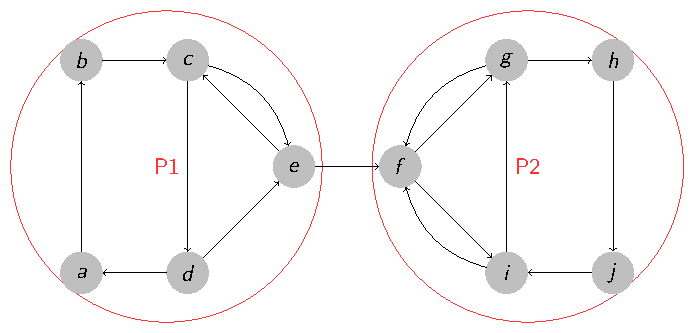
\includegraphics[height=1.2in,width=\columnwidth,trim={0 0 0 0},clip]{resources/contre_exemple}
					}; 
					\node[inner sep=-10pt,visible on=<3->](expressions) at (-1.3,-1.8) {AG\(f\)};             
			
					\end{tikzpicture}
				\end{figure}
			\end{column}
		
         \begin{column}{0.7\textwidth}
         	
         	\begin{block}{Problèmes}
         		\begin{itemize}
         		\item Distribution statique.% la distribution reste intacte tout au long du model cheking
         		\item L'équilibrage peut être dégradé.% pourai entrainer un nombre elever de communications
         	%
         		\item La puissance des machines non exploitée.% il peut y avoir des machines qui effetue peut de calcule alors que les autres un nombre elevé de calcul         		
         	 \end{itemize}
           \end{block}
         \end{column}
		\end{columns}
 \vspace{0.5cm}
\textbf{ Minimisation des transitions externes \color{red} $\stackrel{?}{\Rightarrow}$ Temps de réponse minimisé}.  
\end{frame}

\subsection{Solution en aval}
\begin{frame}
	\centering
	\vspace{2.2cm}       
	\Huge 
	\textbf{Solution en aval}
	%chercher a surcharger une machine faira qu'augmenter le temps de la verification
\end{frame}

\begin{frame}{title sub section}
  
  
  
\begin{center}
	\begin{columns}
		\begin{column}{\textwidth}
			\begin{figure}				
				\begin{tikzpicture}		
				\only<1-1>
				{
					\node [inner sep=-10pt]
					{
						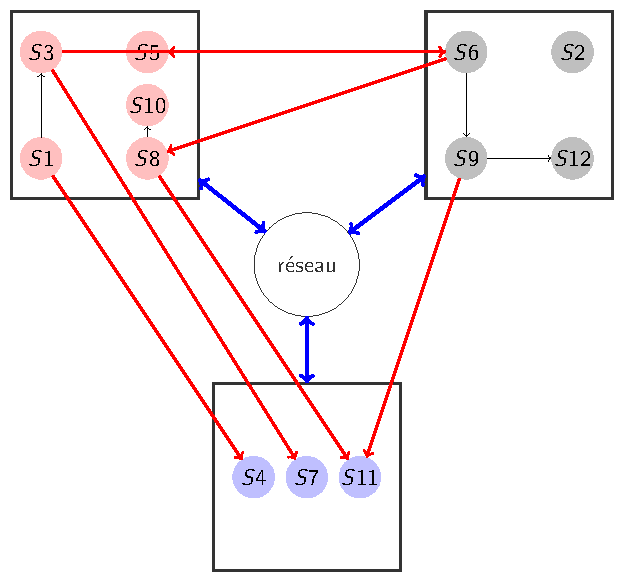
\includegraphics[height=1.8in,width=0.7\columnwidth,trim={0 0 0 0},clip]{resources/benstira/0001}
					};              
				}
			\only<2-2>
			{
				\node [inner sep=-10pt]
				{
					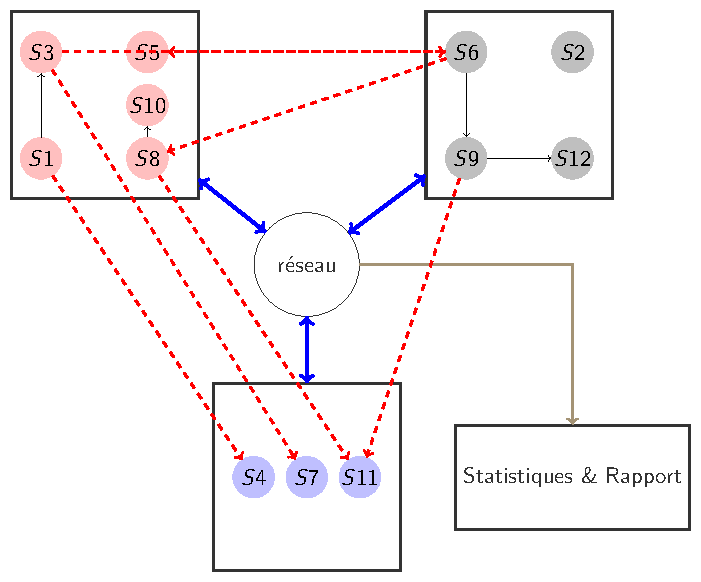
\includegraphics[height=1.8in,width=0.7\columnwidth,trim={0 0 0 0},clip]{resources/benstira/0002}
				};              
			}
			\only<3-3>
			{
				\node [inner sep=-10pt]
				{
					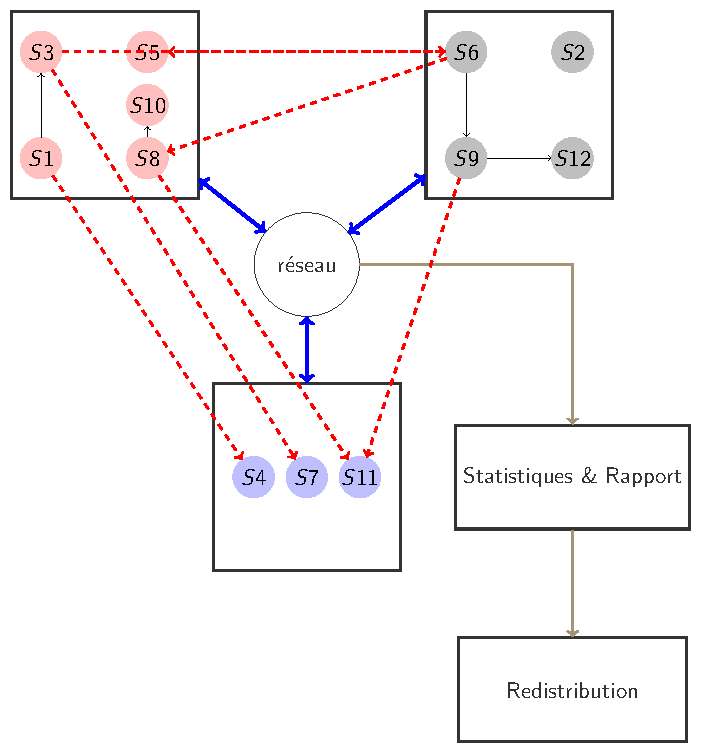
\includegraphics[height=2in,width=0.7\columnwidth,trim={0 0 0 0},clip]{resources/benstira/0003}
				};              
			}
			\only<4-4>
			{
				\node [inner sep=-10pt]
				{
					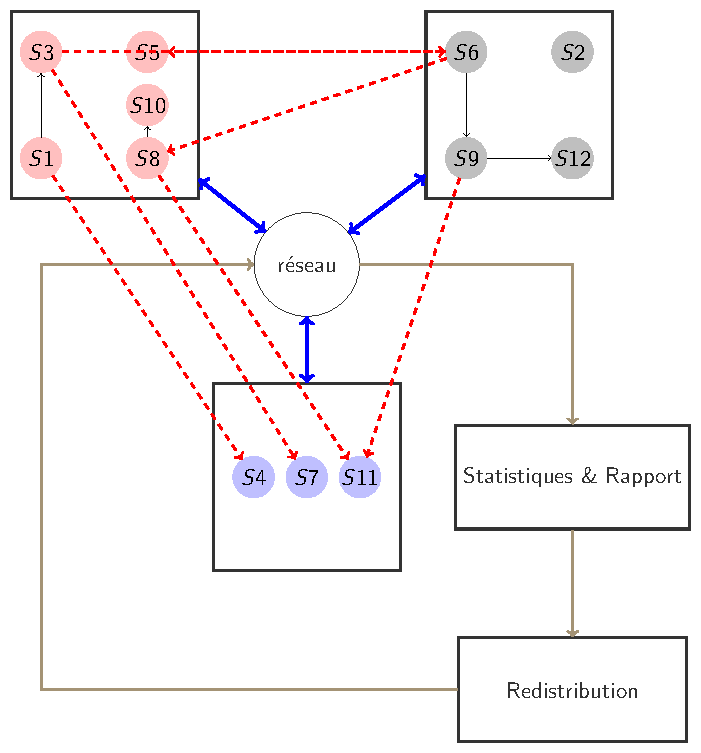
\includegraphics[height=2in,width=0.7\columnwidth,trim={0 0 0 0},clip]{resources/benstira/0004}
				};              
			}		
				\end{tikzpicture}				
				
			\end{figure}
		\end{column}
	\end{columns}
\end{center}
\end{frame}

\begin{frame}
	\centering
	\vspace{2.2cm}       
	\Huge 
	\textbf{Critiques}	
\end{frame}

\begin{frame}{tite subsection}
\vspace{-10pt}
\begin{block}{Critiques}
	\vspace{-15pt}
	\begin{columns}
		\begin{column}{\textwidth}
			\begin{itemize}
				\item Minimisations des transitions externes.
				\item Duplications et Migrations basées sur les transitions.
				\item Certains machines peuvent être surchargées de calcul ou de stockage.
				\item Duplication de certains états est sans intérêt.% sinon le model checking sera faux
			\end{itemize}
		\end{column}
	\end{columns}

	\begin{columns}
		\begin{column}{0.3\textwidth}
			\centering
			\begin{figure}				
				\begin{tikzpicture}		
					\only<1-1>
					{
						\node [inner sep=-10pt]
						{
							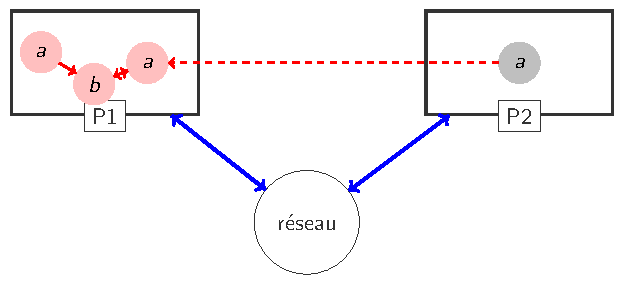
\includegraphics[height=1.2in,width=\columnwidth,trim={0 0 0 0},clip]{resources/benstira/critque1}
						};              
					}
					
					\node [inner sep=-10pt,visible on=<2-2>]
					{
						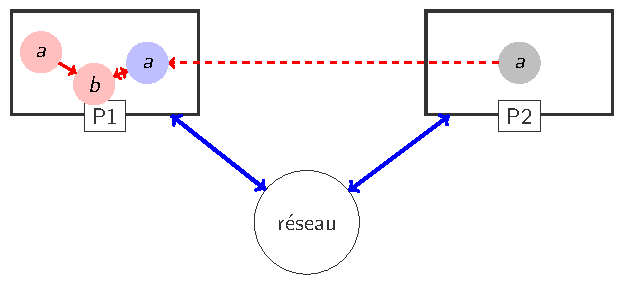
\includegraphics[height=1.2in,width=\columnwidth,trim={0 0 0 0},clip]{resources/benstira/critque2}
					};  
				
					\node [inner sep=-10pt,visible on=<3-3>]
					{
						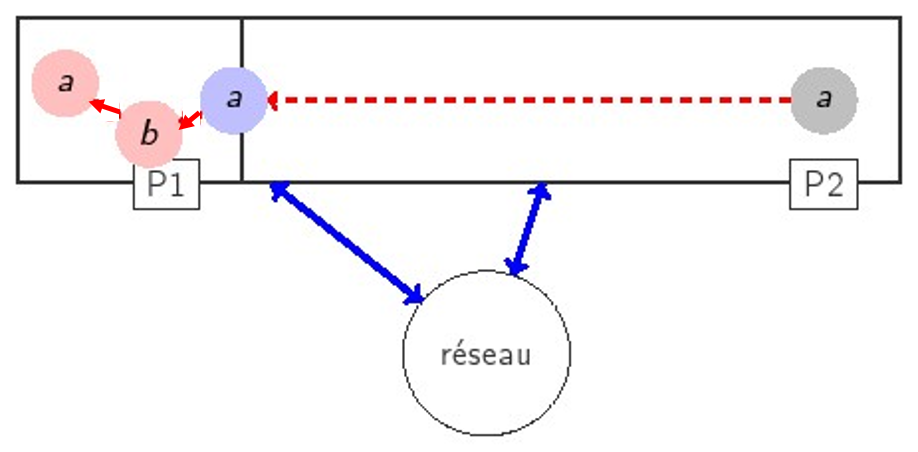
\includegraphics[height=1.2in,width=\columnwidth,trim={0 0 0 0},clip]{resources/benstira/critque3}
					};                
			% question est ce que le temps est amelioré? si oui le model checking sera fausse, sinon la duplication n'a rien servi
				\end{tikzpicture}				
			\end{figure}
		\end{column}
		\begin{column}{0.7\textwidth}
			\begin{itemize}
				\item AG(a)
				\item Si 0.45 < L/$N_t$ ≤ 0.75, alors dupliqué \color{red}{\tiny \citep{BENSETIRA2017}}.
			\end{itemize}
		\end{column}
	\end{columns}
\end{block}
\end{frame}

\subsection{Partitionnent}
\begin{frame}{tite subsection}
\vspace{-10pt}
\begin{block}{Critiques}
	\vspace{-15pt}
	\begin{columns}
		\begin{column}{\textwidth}
			\begin{itemize}
				\item Minimisations des transitions externes.
				\item Duplications et Migrations basées sur les transitions.
				\item Certains machines peuvent être surchargées de calcul ou de stockage.
				\item Duplication de certains états est sans intérêt.% sinon le model checking sera faux
			\end{itemize}
		\end{column}
	\end{columns}
	
\end{block}
\end{frame}

	\section{Contribution}

% nous allons trouver un compromis entre le temps d'execution et l'equilibrage de charge
%\begin{frame}
%\centering
%	\vspace{2.2cm}       
%	\Huge 
%	\textbf{Pourquoi \\la réduction des transitions externes \\et\\ l'équilibrage des états \\n'aide pas le model checking ?}	
%\end{frame}

% avant tout, presentons les point de partitions
%tout partition outre les point que la formule n'est pas verifier initialement entrainera un nombre de calcule. les exemples precedents le demontre.

%il peut arriver que les machine ne peuvent pas supporter ces etats par leur nombres
%le mieux est de le surcharger en calcule ou en stockage que les deux en meme temps
\subsection{Points de partitions}
\begin{frame}{Définition}
  \centering
   \begin{columns}
   	\begin{column}{0.8\textwidth}
   		\vspace{-20pt}
   		\begin{figure}				
   			\begin{tikzpicture}		
   			\only<1-1>
   			{
   				\node [inner sep=-10pt]
   				{
   					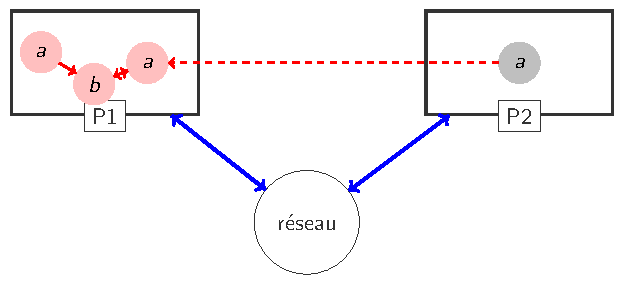
\includegraphics[height=1.2in,width=\columnwidth,trim={0 0 0 0},clip]{resources/benstira/critque1}
   				};              
   			}
   			
   			\node [inner sep=-10pt,visible on=<2->]
   			{
   				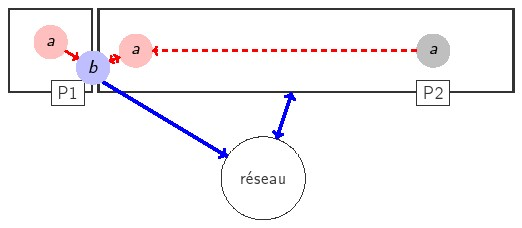
\includegraphics[height=1.2in,width=\columnwidth,trim={0 0 0 0},clip]{resources/pointpartition}
   			};
   		
   			\end{tikzpicture}				
   		\end{figure}
   	\end{column}   	
   \end{columns}

\begin{columns}
	\begin{column}{0.8\textwidth}
		\vspace{15pt}
		\begin{figure}				
			\begin{tikzpicture}	
			\node [inner sep=-10pt,visible on=<3->]
			{
				
\includegraphics[height=1in,width=0.5\columnwidth,trim={0 0 0 0},clip]{resources/pc}
			};			
			\end{tikzpicture}				
		\end{figure}
	\end{column}   	
\end{columns}
\end{frame}

\subsection{Équilibre de Nash}
\begin{frame}{Définition}
\centering
\vspace{-20pt}
\begin{columns}
	\begin{column}{0.3\textwidth}
		\begin{figure}
			\centering
			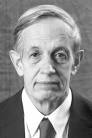
\includegraphics[width=\linewidth]{resources/nash}
		\end{figure}
		
	\end{column}
	\begin{column}{0.7\textwidth}
		\begin{itemize}
			\item Une situation o\`{u} adopte la meilleure réponse du choix des autres.
			\item Il lui a valu le  \textbf{Prix Nobel}  d'économie en 1994.
			%L'existence d'un équilibre n'implique pas que celui-ci soit nécessairement optimal
		\end{itemize}
	\centering
	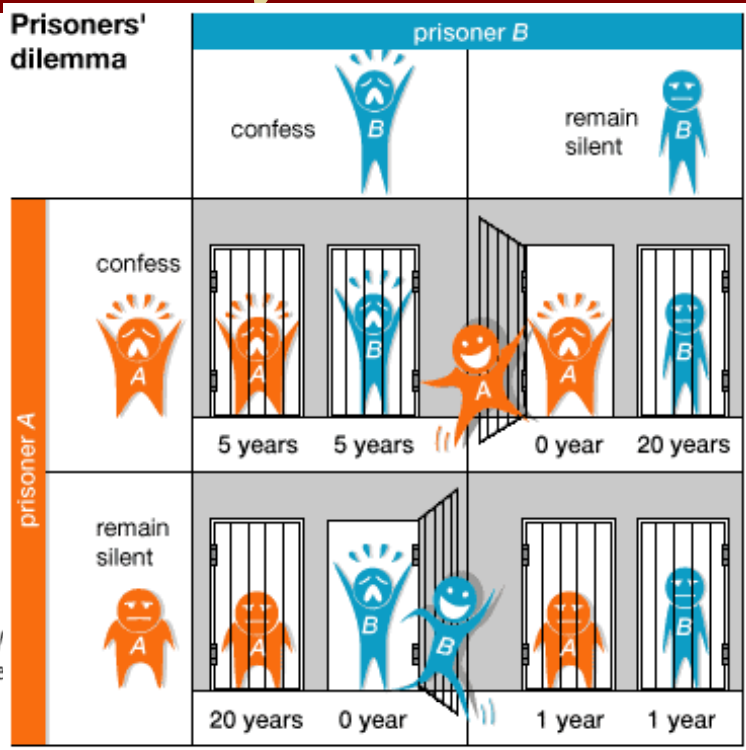
\includegraphics[width=0.5\linewidth]{resources/prisonier}
	\end{column}   	
\end{columns}
\end{frame}


%nous comptons utiliser cette philosophie pour equilibrer le temps de la verification tout en degradant le stockage

\subsection{Stratégie de Distribution}
\begin{frame}{title subsection}
\centering
\vspace{-20pt}
\begin{columns}
	\begin{column}{1\textwidth}
		\begin{figure}
			\centering
			\begin{tikzpicture}	
			\node [inner sep=-10pt,visible on=<1-1>]
			{
				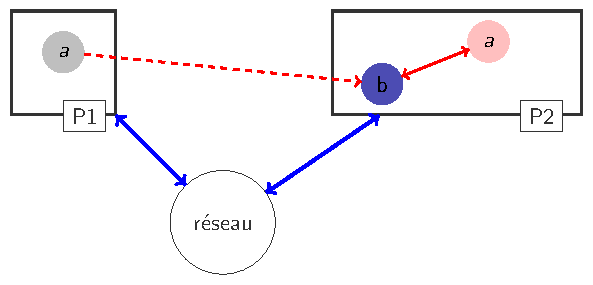
\includegraphics[width=\columnwidth,trim={0 0 0 0},clip]{resources/d1}
			};	
			\node [inner sep=-10pt,visible on=<2-2>]
			{
				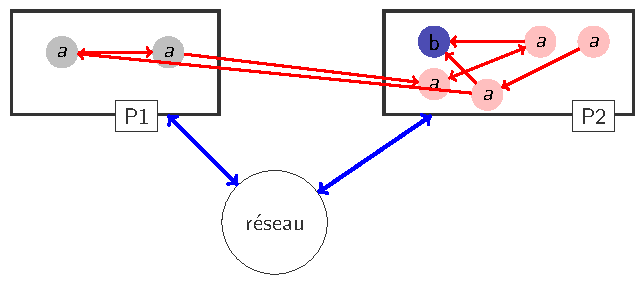
\includegraphics[width=\columnwidth,trim={0 0 0 0},clip]{resources/d2}
			};			
			 
			 \node [inner sep=-10pt,visible on=<3-3>]
			 {
			 	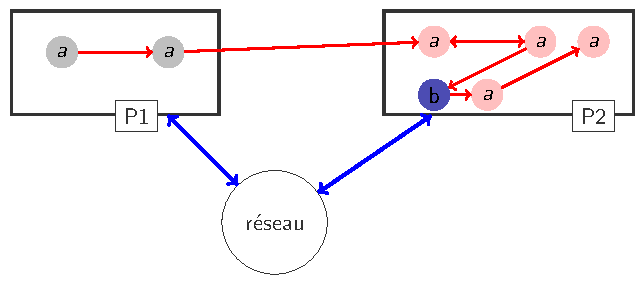
\includegraphics[width=\columnwidth,trim={0 0 0 0},clip]{resources/d3}
			 };	
		 
		 	\node [inner sep=-10pt,visible on=<4-4>]
		 	{
		 		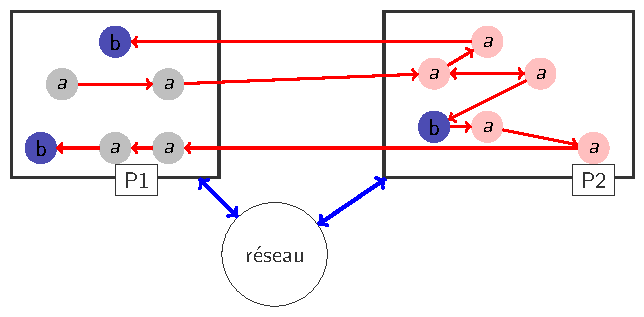
\includegraphics[width=\columnwidth,trim={0 0 0 0},clip]{resources/d5}
		 	};	
	 	
	 	    \node [inner sep=-10pt,visible on=<5-5>]
	 	    {
	 	    	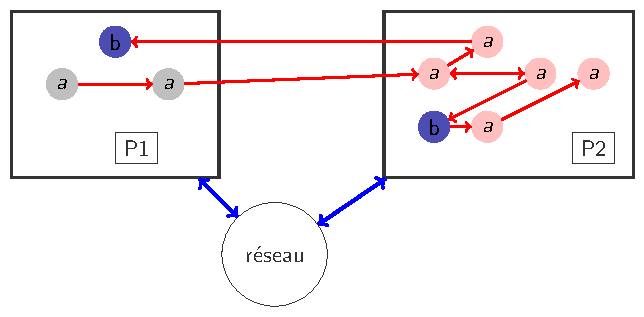
\includegraphics[width=\columnwidth,trim={0 0 0 0},clip]{resources/d4}
	 	    };	
 	    
 	    	\node [inner sep=-10pt,visible on=<6-6>]
 	    	{
 	    		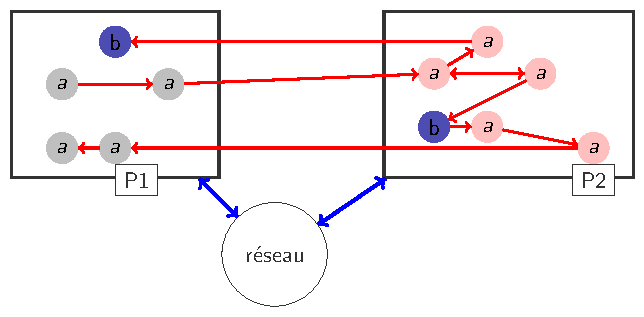
\includegraphics[width=\columnwidth,trim={0 0 0 0},clip]{resources/d6}
 	    	};	
     	
     		\node [inner sep=-10pt,visible on=<7-7>]
     		{
     			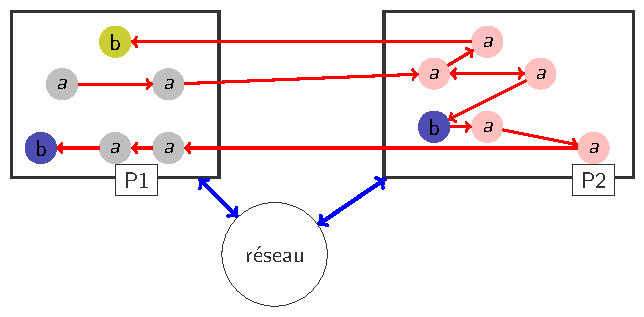
\includegraphics[width=\columnwidth,trim={0 0 0 0},clip]{resources/d7}
     		};	
     	
     		\node [inner sep=-10pt,visible on=<8-8>]
     		{
     			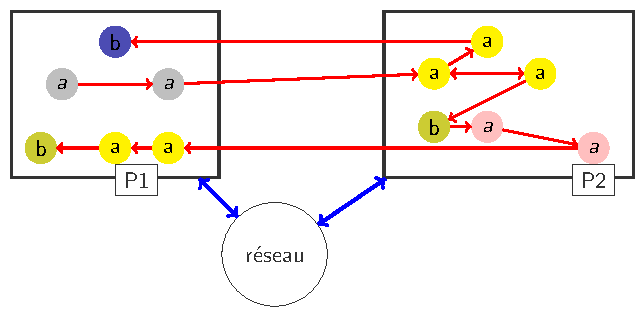
\includegraphics[width=\columnwidth,trim={0 0 0 0},clip]{resources/d8}
     		};	
     	
			\end{tikzpicture}
		\end{figure}		
	\end{column} 
	
\end{columns}
\end{frame}
%nous comptons a realiser une meilleur partion
\subsection{Model checking par déduction}
\begin{frame}{title subsection}
	\begin{block}
	
	\begin{itemize}
		\item Notion de duplicata
		\item Déduit la valeur logique des duplicatas
		\item Minimise le taux de communications
	\end{itemize}
	\end{block}
\end{frame}

%ces deux approche permet d'accelerer le temps de la verification d'une propriete 
	\section{Conclusion}
\subsection{Conclusion}
\begin{frame}{Conclusion}
 
\end{frame}

\subsection{Perspectives}
\begin{frame}{Perspectives}
\begin{block}{Perspectives}
	\begin{itemize}[<+->]
		\transdissolve
		\transduration{2}
		\item   Explorée les différentes stratégies de la théorie de jeux pour apporter des améliorations supplémentaires à notre stratégie afin d’aboutir à une meilleur stratégie de distribution.
		\item  Extraire un modèle de partitionnement basé sur le machine learning à partir des différentes statistiques générées durant l’exécution du model cheking.
	\end{itemize}
 
\end{block}
\end{frame}


\begin{frame}
\begin{itemize}[<+->]
	\transdissolve
	\transduration{2}
	\item Large number of possible parameter-value combinations
	\item Hard to find the optimal parameters
	\item Which parameters should be changed and by how much. 
	\item muliticollinearity or high correlation between parameter values
	\item Which criteria for evaluating the difference between observed and 
	simulated runoff.
\end{itemize}
{\tiny }\end{frame}
\part{\part{title}}
%\pgfdeclarelayer{background}
\pgfsetlayers{background,main}

\begin{frame}
\begin{figure}
	\begin{tikzpicture}[->,scale=1.8, auto,swap]
	% Draw the vertices. First you define a list.
	\foreach \pos/\name in {{(0,0)/a}, {(0,2)/b}, {(1,2)/c},
		{(1,0)/d}, {(2,1)/e}, {(3,1)/f}, 
		{(4,2)/g}, {(5,2)/h}, {(4,0)/i},
		{(5,0)/j}}
	\node[vertex] (\name) at \pos {$\name$};
	
	% Connect vertices with edges and draw weights
	\foreach \source/ \dest /\pos in {a/b/, b/c/, c/d/, d/a/,
		c/e/bend left, d/e/, e/c/,
		e/f/, f/g/, f/i/,
		g/f/bend right, i/f/bend left,
		g/h/, h/j/, j/i/, i/g/}
	\path (\source) edge [\pos] node {} (\dest);
	
	% Start animating the edge selection. 
	% For convenience we use a background layer to 
	% highlight edges. This way we don't have to worry about 
	% the highlighting covering weight labels. 
	\begin{pgfonlayer}{background}
	\foreach \source / \dest / \fr / \pos in {d/a/1/,
		a/b/2/, b/c/3/, c/d/4/, d/e/5/, e/c/6/, 
		c/e/7/bend left, e/f/8/, f/g/9/,
		g/f/10/bend right, f/i/11/, i/g/12/, g/h/13/, 
		h/j/14/, j/i/15/, i/f/16/bend left}
	\path<\fr->[selected edge] (\source.center) edge 
	[\pos] node {} (\dest.center);
	\end{pgfonlayer}
	\end{tikzpicture}
\end{figure}
\end{frame}

\end{document}